% Created 2020-05-11 Mon 17:26
% Intended LaTeX compiler: pdflatex
\documentclass[11pt]{article}
\usepackage[utf8]{inputenc}
\usepackage[T1]{fontenc}
\usepackage{graphicx}
\usepackage{grffile}
\usepackage{longtable}
\usepackage{wrapfig}
\usepackage{rotating}
\usepackage[normalem]{ulem}
\usepackage{amsmath}
\usepackage{textcomp}
\usepackage{amssymb}
\usepackage{capt-of}
\usepackage{hyperref}
\usepackage{relsize}
\usepackage{graphicx}
\usepackage{appendix}
\graphicspath{ {/home/matvey/writ/bio-ia/} }
\usepackage{setspace}
\usepackage{mathtools}
\doublespacing
\date{\today}
\title{}
\hypersetup{
 pdfauthor={},
 pdftitle={},
 pdfkeywords={},
 pdfsubject={},
 pdfcreator={Emacs 26.3 (Org mode 9.3.6)}, 
 pdflang={English}}
\begin{document}

\begin{center}
\huge
BIOLOGY HL INTERNAL ASSESSMENT

\large
\textbf{Research Question}:

Are the double haploids produced by in vitro selection resistant to Fusarium head blight - is there a statistically significant difference between the toxin and control groups?

\textbf{Number of pages}: 22

\textbf{Done by}: Matvey Ryabov

\textbf{Candidate number}: 000556-0010

\textbf{School}: Winston Churchill High School, Lethbridge Alberta 
\end{center}
\pagebreak
\tableofcontents
\section{Research Question}
\label{sec:org3220863}
Are the double haploids produced by in vitro selection resistant to Fusarium head blight - is there a statistically significant difference between the toxin and control groups?

\section{Background Research}
\label{sec:org6c31159}
Fusarium head blight (FHB) is a serious problem to farmers world wide. It costs hundreds of millions of dollars annually in lost yield \cite{wilson2018economic} as farmers are forced
to throw out contaminated crop. It is a disease 
caused by a group of trichothecene mycotoxin producing \emph{Fusarium} species which harm plant growth
and contaminate products. Beer made from contaminated cereals is too foamy \cite{d1998pesticide} and 
bread made from contaminated flour loses its loaf shape \cite{article}. Moreover, humans and animals that consume contaminated cereals - especially those contaminated by the more
dangerous \emph{Fusarium graminearum} - suffer adverse health effects such as anything from gastrointestinal irritation to immune suppression \cite{korosteleva2009effects}. 
Some scientists also believe that consumption of trichothecene mycotoxins can potentially result in a higher chance of developing cancer due to their suppression
of immune protection against tumor development \cite{berek2001effects}. 

\begin{figure}[h]
\centering
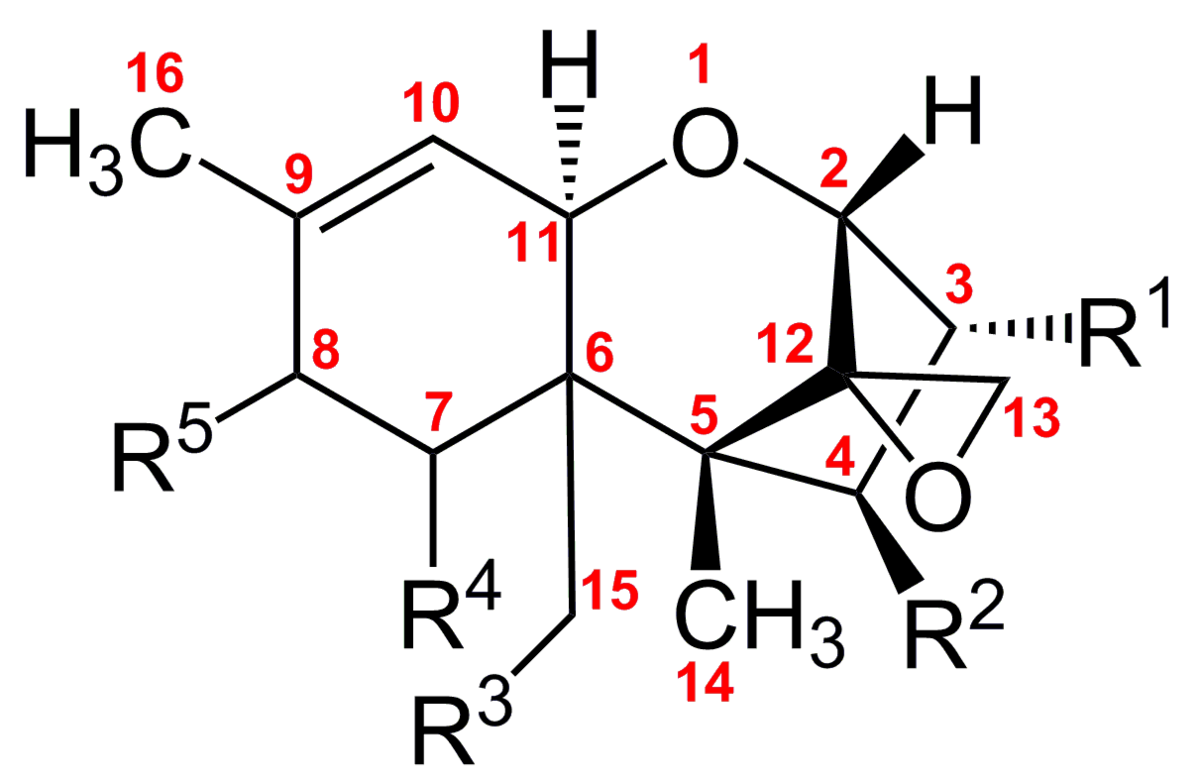
\includegraphics[width=\textwidth]{trich}
\caption{tricothecene mycotoxin}
\end{figure}

Since FHB has such effects - economic cost, adverse health effects, effects on product quality - scientists have been looking for ways to combat this disease.
A potential solution might be the use of pesticides but this has its drawbacks. For example, the fungus can develop resistance to the pesticide making the pesticide less efficient and perhaps 
requiring a new pesticide to be developed. 
Also, pesticides are toxic themselves and are thus dangerous. To mitigate risks of pesticides getting into our food, we have to apply pesticides to the plant while it is in its tillering stage 
rather than in its flowering stage. This means that in its flowering stage, the plant still has a chance of developing
FHB  - thus ruining a yield of crop or at least making the pesticide not fully effective. Since it would be
more efficient to have a plant that is naturally resistant to FHB rather than requiring pesticides, scientists have been looking at
breeding FHB resistant plants. One way of doing this is by the use of in vitro selection. This means that microspores of a plant are exposed
to toxins (trichothecenes) during in vitro making some of the microspores die but the toxin resistant microspores survive. These microspores turn into double haploids (either naturally or through laboratory means) which can be planted and grown. 
Studies have found that there are genetic traits that allow for resistance to trichothecene \cite{foroud2012differential}. This would suggest that it should be possible 
to use in vitro selection to select for these resistance-allowing traits. This investigation looks at determining whether in vitro selection can be used
to select \emph{Fusarium} resistant wheat - are the double haploids produced by in vitro selection resistant to FHB? 

\section{Hypothesis}
\label{sec:orge24c77c}
It can be predicted that the trichothecene resistance is present in the genetic code of the double haploids that underwent in vitro selection (well the microspores did - but the double haploids were developed from them), and thus, the severity/incidence of FHB damage should be 
lower in the plants of the toxin group - vs. the control group which didn't undergo in vitro selection.

This is because the traits allowing the microspores to survive in vitro selection, would be passed onto the double haploids. 

Therefore, the hypotheses for the statistical testing are as follows:

\textbf{Null Hypothesis:} The control and the toxin groups of the L15038 cross are statistically equal - the difference between a randomly selected
value from group 1 and group 2 is not large enough to be considered statistically significant.

\textbf{Alternative Hypothesis}: The control and the toxin groups of the L15038 cross are not statistically equal - the difference between a randomly
selected value from group 1 and group 2 is large enough to be considered statistically significant.
\section{Materials:}
\label{sec:orgd0b14d4}
\begin{itemize}
\item Gnumeric (open-source alternative to Microsoft Excel) is used for data cleaning and formatting.
\item R is used to both draw the graphs and perform the statistical analysis.
\item Statistics Kingdom website was used initially to get an interactive understanding of the test \url{http://www.statskingdom.com/170median\_mann\_whitney.html} and Statistics at the Bench \cite{bremer_doerge_2010} was used as a later reference - especially for the trial investigation.
\item Field Dataset which has data on several populations of toxic \& control groups with several responding observation sets. Obtained with permission from the Nora Foroud lab.
\end{itemize}
\subsection{Dataset Used:}
\label{sec:org856908f}
The dataset consists of FHB effect data for several populations (different crosses) of spring wheat. 
Within this data, there are two groups - the control and the toxin group. The toxin group data was obtained via microspores that were collected, in vitro selected
for toxin resistance, developed into double haploids, and then grown into adult plants. The data consists of three
variables (effects): VRI\% (incidence * severity of FHB), FDK\% (percentage of \emph{Fusarium} damaged kernels), and the chemical amount of toxins (more specifically deoxynivalenol) present in the grain. For the sake of this experiment, I used data from one cross of spring wheat (L15038) while there were three in the dataset.
I did this to get rid of the variation resulting from genetic variation between the crosses.    
\section{Methodology \& Trial Investigation:}
\label{sec:org3512a93}
\subsection{Statistical Test Chosen:}
\label{sec:orgb9f5588}
Because my data cannot satisfy the assumptions required for a Student T-test (equal variance in standard deviation, normal distribution, and equal sample size) nor
the assumptions for a Welch's Modified T-test (normal distribution), I decided to use a different
test called the Matt Whitney U Test (or the Wilcoxon Rank Sum Test). This test is 
used to test whether two samples are likely to derive from the same population \cite{manwhit} (i.e., that the two populations have the same shape) by 'comparing the medians' of the two populations.

The Matt Whitney U Test equation is given below \cite{bremer_doerge_2010}:
\begin{equation}
U = n_{1}n_{2} + \frac{n_{1}(n_{1}+1)}{2} - R_1 \sim N\left(\mu = \frac{n_{1}n_{2}}{2}, \sigma = \sqrt{\frac{n_{1}n_{2}(n_{1} + n_{2} + 1)}{12}}\right)
\end{equation}

Where R\textsubscript{1} is the rank sum of group 1, n\textsubscript{1} is the number of individuals group one, and n\textsubscript{2} is the number of individuals in group two.
\subsection{Test Procedure:}
\label{sec:orgde6489b}
\begin{enumerate}
\item VRI\%, FDK\%, and DON ppm data was isolated from the 'metadata' columns.
\item Each variable observation was ranked. Ties between repeated observations of the same magnitude are broken by averaging their ranks.
\item A rank sum was calculated for each group (although only one or the other needs to be used).
\item The U statistic is calculated with the Matt Whitney U Test equation in the section above (1).
\item Since this statistic has approximately a normal distribution, it is possible to calculate a mean \(\mu\) and a standard deviation \(\sigma\) using the equation in the section above (1).
\item A \textit{p}-value for this test can be obtained using a normal distribution with the values calculated in step 5 - as defined by equation in section above (1).
\end{enumerate}
\subsection{Trial Investigation:}
\label{sec:orgb82a222}
The following trial investigation was conducted with a sub-sample of the dataset I used. I randomly selected 20 control VRI\% samples and 12 toxin VRI\% samples - this control to toxin ratio is roughly the same as the actual ratio of the population. 
Although this small sample size is likely not a good representation of the population, I am only using this to explain
the test methodology. A significance level (\(\alpha\)) of 0.05 was used.

\begin{figure}[h]
\centering
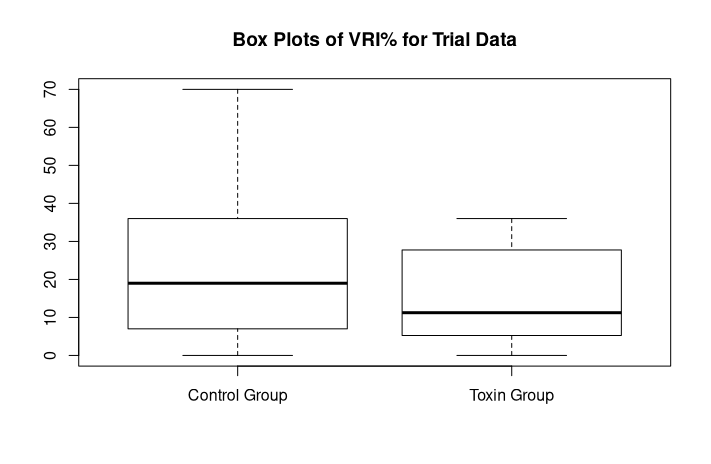
\includegraphics[width=\textwidth]{test}
\caption{Trial investigation data box plot}
\end{figure}


% latex table generated in R 3.6.3 by xtable 1.8-4 package
% Wed Mar 18 19:51:11 2020
\begin{table}[ht]
\centering
\begin{tabular}{rrlr}
  \hline
 & VRI\% Observation & Population & Rank \\ 
  \hline
1 & 0.00 & Control & 1.50 \\ 
  2 & 18.00 & Control & 18.00 \\ 
  3 & 10.50 & Control & 13.50 \\ 
  4 & 0.25 & Control & 3.00 \\ 
  5 & 34.00 & Control & 25.50 \\ 
  6 & 20.00 & Control & 19.00 \\ 
  7 & 54.00 & Control & 31.00 \\ 
  8 & 6.00 & Control & 8.00 \\ 
  9 & 49.50 & Control & 29.00 \\ 
  10 & 29.75 & Control & 23.00 \\ 
  11 & 38.00 & Control & 28.00 \\ 
  12 & 2.00 & Control & 4.00 \\ 
  13 & 8.00 & Control & 11.00 \\ 
  14 & 22.00 & Control & 20.00 \\ 
  15 & 15.00 & Control & 17.00 \\ 
  16 & 70.00 & Control & 32.00 \\ 
  17 & 6.00 & Control & 8.00 \\ 
  18 & 50.00 & Control & 30.00 \\ 
  19 & 24.00 & Control & 21.50 \\ 
  20 & 9.00 & Control & 12.00 \\ 
  21 & 7.50 & Toxin & 10.00 \\ 
  22 & 10.50 & Toxin & 13.50 \\ 
  23 & 0.00 & Toxin & 1.50 \\ 
  24 & 31.50 & Toxin & 24.00 \\ 
  25 & 36.00 & Toxin & 27.00 \\ 
  26 & 13.75 & Toxin & 16.00 \\ 
  27 & 12.00 & Toxin & 15.00 \\ 
  28 & 4.50 & Toxin & 6.00 \\ 
  29 & 6.00 & Toxin & 8.00 \\ 
  30 & 2.50 & Toxin & 5.00 \\ 
  31 & 34.00 & Toxin & 25.50 \\ 
  32 & 24.00 & Toxin & 21.50 \\ 
   \hline
\end{tabular}
\caption{Trial investigation data table}
\end{table}
 

The rank sum for the control population is R\textsubscript{1} = 355. The rank sum for the toxin population is R\textsubscript{2} = 173. Compute the U-test statistic as:

\begin{equation*}
U = (20)(12) + \frac{(20)(20 + 1)}{2} - 355 = 95
\end{equation*}

The test statistic has a normal distribution with mean 

\begin{equation*}
\mu{} = \frac{(20)(12)}{2} = 120
\end{equation*}

and a standard deviation of

\begin{equation*}
\sigma{} = \sqrt{\frac{(20)(12)((20) + (12) + 1)}{12}} = 25.6905.
\end{equation*}

The \textit{p}-value can be calculated with the R command pnorm(-abs(95-120), 120, 25.6905) which yields a \textit{p}-value of 8.3E-09. Since the \textit{p}-value is smaller than the significance level \(\alpha\),
we reject the null hypothesis and state that there is a statistically significant difference between the toxin and control groups. The investigation will follow the same methodology except it will be largely automated using R (using the wilcox.test() function). The code used for the next section will be included in the appendix.
\section{Investigation and Results:}
\label{sec:orgd4f2a86}
\subsection{VRI\% Test Results:}
\label{sec:org0a9e025}
\noindent
U statistic for control group: 2941

\noindent
U statistic for toxin group: 3715

\noindent
\textit{p}-value obtained: 0.2064

A \textit{p}-value of such magnitude means the probability of rejecting a correct null hypothesis would be too large. Thus we accept the null hypothesis and state that the two groups don't have a statistically significant difference in terms of VRI\% (incidence * severity).

\begin{figure}[h]
\centering
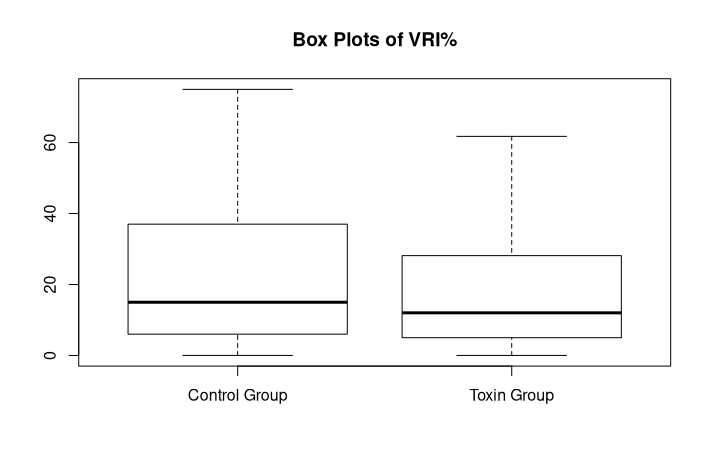
\includegraphics[width=\textwidth]{VRI}
\caption{Box plot for VRI data}
\end{figure}

\subsection{FDK\% Test Results:}
\label{sec:org328a8c3}
\begin{figure}[h]
\centering
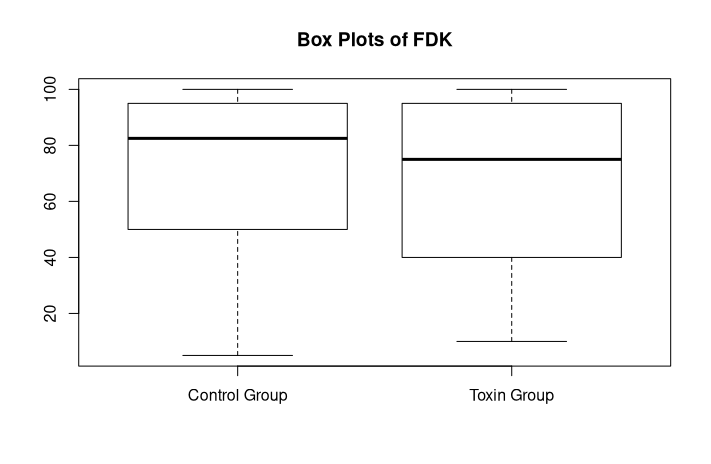
\includegraphics[width=\textwidth]{FDK}
\caption{Box plot for FDK data}
\end{figure}

\noindent
U statistic for control group: 2932

\noindent
U statistic for toxin group: 3724

\noindent
\textit{p}-value obtained: 0.1930

A \textit{p}-value of this magnitude means the probability of rejecting a correct null hypothesis would be too large. Thus we accept the null hypothesis and state that the two groups don't have a statistically significant difference in terms of their percentages of \emph{Fusarium} damaged kernels.
\subsection{DON ppm Test Results:}
\label{sec:org8c0ba37}
\begin{figure}[h]
\centering
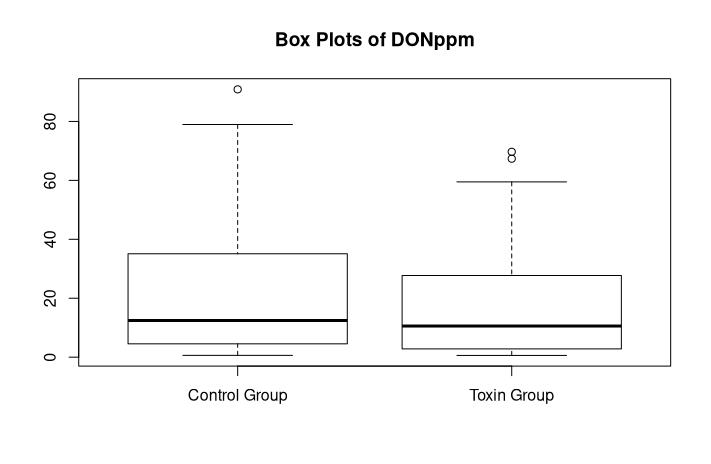
\includegraphics[width=\textwidth]{DONppm}
\caption{Box plot for DON ppm data}
\end{figure}

The DON ppm data had 3 total outliers. These were determined using the Tukey Fence method and were removed automatically.

\noindent
U statistic for control group: 2683

\noindent
U statistic for toxin group: 3703

\noindent
\textit{p}-value obtained: 0.865

A \textit{p}-value of this magnitude means the probability of rejecting a correct null hypothesis would be too large. Thus we accept the null hypothesis and state that the two groups don't have a statistically significant difference in terms of the chemical amount of trichothecene toxins present in their grains.
\section{Analysis \& Conclusion:}
\label{sec:org885bafd}
To restate the research question: \textbf{Are the double haploids produced by in vitro selection resistant to Fusarium head blight - is there a statistically significant difference between the toxin and control groups?}

For all three effect variables, there was no statistically significant difference observed in the L15038 cross. The \textit{p}-value was larger than the \(\alpha\) value for each. 

In conclusion, this investigation has found that there isn't a statistically significant difference between the toxin and control groups in terms of FHB effect observations - for at least the L15038 cross. This does not support my alternative hypothesis and I must accept the null hypothesis for all of the effects tested (VRI\%, FDK\%, and DON ppm).
A biological explanation for the lack of a statistically significant difference could be that the variance present between individual double haploid lines would make it difficult to
observe a difference - there might be significant variation in resistance 'ability' even among members of the same cross. 
Since the microspores used for this experiment were obtained from a hybrid cross (L15038), each chromosome (in a homologous pair) in the original (F1) cell came from a different parent.  This means that their homologous chromosomes contain genes in the same order, but, don't necessarily have the same alleles.
This means that when these homologous chromosomes separate during meiosis, the resulting haploid cell could have either of the alleles - if the alleles are indeed different. Having the possibility of different arrangements of
alleles creates variation. Since \emph{Fusarium} resistance is a polygenic trait \cite{foroud2012differential} and is quantitative \cite{kumar2007identification}, there is added complexity which when combined with this variance in alleles, could be significantly affecting our ability to find a statistically significant difference between the two groups.     
\section{Evaluation:}
\label{sec:org2a9b92c}
\begin{center}
\begin{tabular}{lll}
\hline
Limitation: & Significance: & Potential Improvement:\\
\hline
\# of DH lines produced \footnotemark & Limits the chances of finding & Treating with embryo\\
 & a resistant genotype. & development improving\\
 &  & chemicals \cite{poster}.\\
\# of crosses tested & Crosses have different genetical & Testing more crosses.\\
 & backgrounds. & \\
The nursery is outside & Lack of control on environmental factors. & Testing in a greenhouse.\\
\hline
\end{tabular}
\end{center}\footnotetext[1]{\label{orgda485b4}Some lines were recalcitrant with the tissue culture.}
To reiterate, this investigation has found that there isn't a statistically significant difference between the control and toxin groups in terms of FHB effects in the L15038 cross. Applying the improvements outlined above could potentially 
make it easier to observe an effect - and a statistically significant difference. Despite there currently being no statistically significant difference, further experimentation is being carried out.
This is because finding a resistant line would be very useful (as outlined in introduction) - and this in vitro method still has potential (especially since only one cross was tested - L15038).  

\bibliography{bio}
\bibliographystyle{unsrt}
\section{Appendix:}
\label{sec:orge5e40b2}
\subsection{R Script Responsible For Matt-Whitney U Test:}
\label{sec:orge0ffc8d}
\begin{verbatim}
library(gdata)
library(xtable)

#W -> the sum of the ranks for positive class?
#if p > a , null hypothesis is accepted - the difference between a randomly 
#selected value 
#from group 1 and group 2 is not big enough to be considered to be 
#statistically significant
#X1 is always control, X2 is always toxin


#Wilcox Test VRI
  #Control Data
x1<-c(0,0,0,0,0,0.25,0.25,0.5,1,1,1,1.5,2,2,2,4,4,4,5,5,5,6,6,6,6,6,6,6,6,6,6,6,6,
7.5,7.5,7.5,8,9,9,9,10,10.5,10.5,10.5,12,12,12,12,12,12,13,15,15,15,16.25,17.5,18,
20,20,21,22,22,22,22.5,24,24,24,25,26,27,28.5,29.75,32,34,34,36,36,36,38,40,40,45,
45,47.5,47.5,47.5,47.5,49.5,50,54,54,54,57,59.5,60,61.75,63,66.5,70,70,70,70,70,75)

  #Toxin Data
x2<-c(0,0,0,0,0,0,0,0.25,2,2.5,3,4,4,4.5,5,5,5,6,6,6,6.25,7.5,7.5,7.5,7.5,7.5,8,9,
9,10.5,10.5,12,12,13.75,14,14,15,20,21,22,22.5,22.5,22.5,22.5,24,24,24.5,26.25,30,
30,31.5,32,34,34,36,36,38.25,40.5,41.25,45,51,54,57,61.75)
wilcox.test(x1, x2, alternative = "two.sided", paired = FALSE, exact = FALSE, 
                correct = TRUE)
boxplot(x1,x2,names=c("Control Group", "Toxin Group"))
title("Box Plots of VRI%")

#Trial investigation
control_trial <- sample(x1, size=20, replace=F)
toxin_trial <- sample(x2, size=12, replace=F)
boxplot(control_trial, toxin_trial, names=c("Control Group", "Toxin Group"))
title("Box Plots of VRI% for Trial Data")
trial_data <- combine(control_trial, toxin_trial, names=c("Control","Toxin"))
trial_data$rank <- rank(trial_data$data, na.last=FALSE, ties.method="average")
names(trial_data) <- c("VRI% Observation", "Population", "Rank")
print(xtable(trial_data, type = "latex", tabular.environment="longtable"), 
                         file ="table.tex", row.names = FALSE)
#Rank Sum Control
sum(trial_data$Rank[1:20])
#Rank Sum Toxin
pnorm(-25, 120, 25.6905)

#Wilcox Test FDK
  #Control Data
x1<-c(5,10,10,20,20,20,20,20,20,25,25,30,30,35,35,40,40,40,40,40,45,50,50,50,50,
50,50,50,50,50,50,55,60,60,60,60,65,65,65,70,70,70,70,70,70,70,70,70,75,80,80,80,
85,85,88.597701,90,90,90,90,90,90,90,90,90,95,95,95,95,95,95,95,95,95,95,95,95,
95,95,95,95,100,100,100,100,100,100,100,100,100,100,100,100,100,100,100,100,100,
100,100,100,100,100,100,100)

  #Toxin Data
x2<-c(10,20,20,20,20,20,20,25,25,25,30,30,30,30,40,40,40,40,50,50,50,50,55,60,60,
60,60,60,70,70,70,75,75,75,80,80,88.597701,88.597701,90,90,90,95,95,95,95,95,95,
95,95,95,95,95,95,95,95,95,95,95,100,100,100,100,100,100)
wilcox.test(x1, x2, alternative = "two.sided", paired = FALSE, 
                exact = FALSE, correct = TRUE)
boxplot(x1,x2,names=c("Control Group", "Toxin Group"))
title("Box Plots of FDK")


#Wilcox Test DON ppm
  #Control Data
x1<-c(0.614476,0.888792,1.119769,1.120836,1.2,1.425799,1.580311,1.718518,1.856635,
1.891906,1.925498,1.929826,2.577703,2.65,2.775984,2.807378,2.980268,2.999115,
3.326483,3.472574,3.500409,3.884181,3.915637,4.049918,4.223999,4.285536,4.749604,
4.898587,5.133321,5.526058,5.774488,5.886955,6.08955,6.157488,6.2,6.317295,6.452412,
6.90394,6.916808,7.058226,7.1,7.205961,7.314642,7.470937,7.621857,8.378225,8.822314,
9.304468,9.480144,9.629332,11.845629,12.266822,12.628974,12.66,12.795816,13.358016,
15.197585,16.145625,16.581646,18.402242,18.93175,23.427736,24.309438,25.019106,
25.499436,26.65426,26.88642,27.69684,28.950617,29.851023,30.127327,31.310614,
31.575228,32.13125,32.615206,32.704927,33.25931,34.125959,36.056148,36.577781,
36.616944,37.929188,38.76385,38.989765,39.712798,41.019588,41.719137,42.985482,
43.064517,43.375339,43.809959,45.961754,47.201307,50.413292,50.595373,51.529422,
61.093009,62.069529,65.24486,67.711618,67.939119,68.70372,78.960075,90.895459)

  #Toxin Data
x2<-c(0.584063,0.603603,0.638811,0.8,1.068102,1.072556,1.094445,1.433779,1.495372,
1.737329,1.811584,1.903887,2.202997,2.248326,2.370205,2.650943,2.955159,3.217394,
3.403908,3.616216,3.630006,3.813682,4.203648,4.612841,4.798336,4.989804,5.569431,
6.203574,6.568003,8.244328,9.76663,10.177096,10.932861,13.645659,13.873584,15.832693,
15.844279,16.589565,19.133919,19.7276,21.567897,22.316369,22.713886,23.378631,
24.393695,25.873869,26.353619,26.424969,28.992688,29.346735,30.489248,32.064561,
35.288046,35.760166,37.462641,41.950031,42.654444,43.844248,45.062117,50.137477,
54.348779,59.495856,67.356837,69.704457)
wilcox.test(x1, x2, alternative = "two.sided", paired = FALSE, 
                exact = FALSE, correct = TRUE)
boxplot(x1,x2,names=c("Control Group", "Toxin Group"))
title("Box Plots of DON ppm")
\end{verbatim}
\end{document}